% Source: graduate-coursework/Research/Intro_to_Agents/slides/From_LLMs_to_Multi_Agent_Systems_slides.tex

\documentclass[border=4pt]{standalone}
\usepackage[T1]{fontenc}
\usepackage{graphicx}
\usepackage{tikz}
\usepackage{xcolor}
\usetikzlibrary{arrows.meta,positioning,shapes.geometric,fit,calc,
                decorations.pathreplacing,backgrounds,patterns,trees}

\definecolor{garnet}{HTML}{73000A}
\definecolor{rose}{HTML}{CC2E40}
\definecolor{atlantic}{HTML}{466A9F}
\definecolor{congaree}{HTML}{1F414D}
\definecolor{horseshoe}{HTML}{65780B}
\definecolor{grass}{HTML}{CED318}
\definecolor{honeycomb}{HTML}{A49137}
\definecolor{warmgrey}{HTML}{676156}
\definecolor{sandstorm}{HTML}{FFF2E3}
\definecolor{bk90}{HTML}{363636}
\definecolor{bk70}{HTML}{5C5C5C}
\definecolor{bk50}{HTML}{A2A2A2}
\definecolor{bk30}{HTML}{C7C7C7}
\definecolor{bk10}{HTML}{ECECEC}

\tikzset{
  agentbox/.style={
    rectangle, draw=#1, fill=#1!8, thick,
    minimum width=2.2cm, minimum height=0.8cm,
    font=\small\sffamily, align=center,
    inner sep=4pt
  },
  agentbox/.default=garnet,
  workerbox/.style={
    rectangle, draw=atlantic, fill=atlantic!8, thick,
    minimum width=1.8cm, minimum height=0.7cm,
    font=\small\sffamily, align=center,
    inner sep=3pt
  },
  tierbox/.style={
    rectangle, draw=#1, fill=#1!5, thick,
    minimum width=6.5cm, minimum height=1.0cm,
    font=\small\sffamily, align=center,
    inner sep=4pt
  },
  tierbox/.default=garnet,
  dataarrow/.style={
    -{Stealth[length=5pt]}, thick, color=#1
  },
  dataarrow/.default=bk70,
  brace/.style={
    decorate, decoration={brace, amplitude=6pt, raise=2pt}, thick, color=#1
  },
  brace/.default=bk50,
  labelnode/.style={
    font=\scriptsize\sffamily, color=bk70
  },
  codebox/.style={rectangle, draw=bk70, fill=bk90, text=white,
    font=\ttfamily\small, inner sep=6pt, align=left, text width=#1},
  codebox/.default=6cm,
  sysprompt/.style={rectangle, draw=rose, dashed, fill=rose!5, thick,
    minimum width=2.0cm, minimum height=0.6cm,
    font=\small\sffamily, align=center, inner sep=3pt},
  tooldef/.style={rectangle, draw=atlantic, fill=atlantic!8, thick,
    minimum width=1.8cm, minimum height=0.6cm,
    font=\small\sffamily, align=center, inner sep=3pt},
  wrapperbox/.style={rectangle, draw=garnet, dashed, thick, fill=garnet!3,
    inner sep=8pt},
  pbar/.style={rectangle, draw=#1, fill=#1!30, thick,
    minimum height=0.3cm, font=\scriptsize\sffamily},
  pbar/.default=horseshoe,
  flag/.style={rectangle, draw=rose, fill=rose!15, thick,
    minimum width=0.8cm, minimum height=0.4cm,
    font=\tiny\sffamily\bfseries},
  failbox/.style={rectangle, draw=rose, fill=rose!10, thick,
    font=\small\sffamily, align=center, inner sep=4pt},
}

\begin{document}
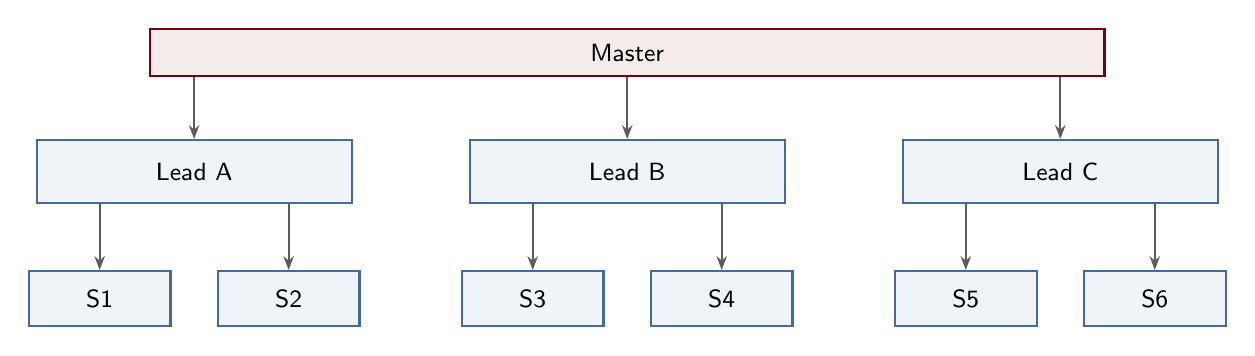
\begin{tikzpicture}[node distance=0.8cm and 0.8cm]
  \node[agentbox=garnet, minimum width=\textwidth, minimum height=0.6cm] (root) {Master};
  \node[agentbox=atlantic, minimum width=4cm] at ([yshift=-1.2cm, xshift=-5.5cm]root.south) (leadA) {Lead A};
  \node[agentbox=atlantic, minimum width=4cm] at ([yshift=-1.2cm]root.south) (leadB) {Lead B};
  \node[agentbox=atlantic, minimum width=4cm] at ([yshift=-1.2cm, xshift=5.5cm]root.south) (leadC) {Lead C};
  \draw[dataarrow] (root.south -| leadA) -- (leadA);
  \draw[dataarrow] (root.south -| leadB) -- (leadB);
  \draw[dataarrow] (root.south -| leadC) -- (leadC);
  \node[workerbox] at ([yshift=-1.2cm, xshift=-1.2cm]leadA.south) (sa1) {S1};
  \node[workerbox] at ([yshift=-1.2cm, xshift=1.2cm]leadA.south) (sa2) {S2};
  \draw[dataarrow] (leadA.south -| sa1) -- (sa1);
  \draw[dataarrow] (leadA.south -| sa2) -- (sa2);
  \node[workerbox] at ([yshift=-1.2cm, xshift=-1.2cm]leadB.south) (sb1) {S3};
  \node[workerbox] at ([yshift=-1.2cm, xshift=1.2cm]leadB.south) (sb2) {S4};
  \draw[dataarrow] (leadB.south -| sb1) -- (sb1);
  \draw[dataarrow] (leadB.south -| sb2) -- (sb2);
  \node[workerbox] at ([yshift=-1.2cm, xshift=-1.2cm]leadC.south) (sc1) {S5};
  \node[workerbox] at ([yshift=-1.2cm, xshift=1.2cm]leadC.south) (sc2) {S6};
  \draw[dataarrow] (leadC.south -| sc1) -- (sc1);
  \draw[dataarrow] (leadC.south -| sc2) -- (sc2);
\end{tikzpicture}
\end{document}
